\documentclass[11pt, a4paper]{article}
\usepackage[utf8]{inputenc}
\usepackage[left=2.35cm, right=3.35cm, top=3.35cm, bottom=3.0cm]{geometry}
\usepackage{amsmath, amssymb, amsthm}
\usepackage[english]{babel}
\usepackage{graphicx}
\usepackage[font={small,it}]{caption}
\graphicspath{ {figures/} }
\usepackage{url}
\usepackage{appendix}
\usepackage{float}
\usepackage{multirow}
\usepackage[bottom]{footmisc}
\usepackage{titling}
\usepackage{subcaption}
\usepackage{wrapfig}
\usepackage[numbered,autolinebreaks,useliterate]{mcode}
\begin{document}

\begin{titlepage}
  \begin{center}
    
    
\includegraphics[scale=1.5]{figures/kuleuven_logo.pdf}~\\[4.5cm]
    \textsc{\Large Master of bioinformatics}\\[0.5cm]

    % Title
    \rule{\linewidth}{0.3mm}\\[0.4cm]
    {\huge \bfseries Support Vector Machines} \\[0.4cm]
    {\large Assignment 2: Function estimation and Time-series prediction} \\[0.4cm]
    \rule{\linewidth}{0.3mm}\\[0.4cm]
    {\large Spring 2016} \\[1.0cm]
    
    % Author and supervisor
    \begin{minipage}{0.4\textwidth}
      \begin{flushleft} \large
        \emph{Author:}\\
	Cedric \textsc{Lood}
      \end{flushleft}
    \end{minipage}
%     %\hfill
    \begin{minipage}{0.4\textwidth}
      \begin{flushright} \large
        \emph{Supervisors:} \\
        Dr. Carlos \textsc{Alaiz}\\
        Dr. Emanuele \textsc{Frandi}\\
        Prof. Johan \textsc{Suykens}\\
        \hfill \newline 
      \end{flushright}
    \end{minipage}
    
    \vfill

    
\includegraphics[scale=0.15]{figures/KUL.jpg}~\\[0.5cm]

    % Bottom of the page
    {\large \today}
    
  \end{center}
\end{titlepage}

\tableofcontents
\newpage

\section*{Context}

The analysis presented in this report was produced for the class of
``Support Vector Machines: methods and applications'' (Spring 2016) at
KU Leuven. The goal is to display understanding of the techniques and
of their practical use. This second report focuses on function
estimation and time series prediction using SVM, and Least-Squares SVM
(LS-SVM). The implementation was done using the MatLab software
(v2015a) and the libraries for LS-SVM developed at KU Leuven.

\section{Support Vector Machine for regression}

\subsection{Datasets}
I experimented with 3 noiseless datasets of 20 observations for this
section, based on the true underlying function shown in figure
\ref{fig:regress_datasets}. I used the ``load dataset'' functionality
of the \emph{uiregress} function to load them and perform the regress:

\begin{lstlisting}
X = (linspace(-5, 5, 20))'; Y = (2.*X + 1)';
save('lin.mat');

X = (linspace(-5,5,20))'; Y = (X.^3 + X.^2 - 1)';
save('poly.mat');

X = (linspace(-pi,pi,20))'; Y = (exp(-X.^2).*sin(10.*X))';
save('sinc.mat');
\end{lstlisting}

\begin{figure}[H]
    \centering
    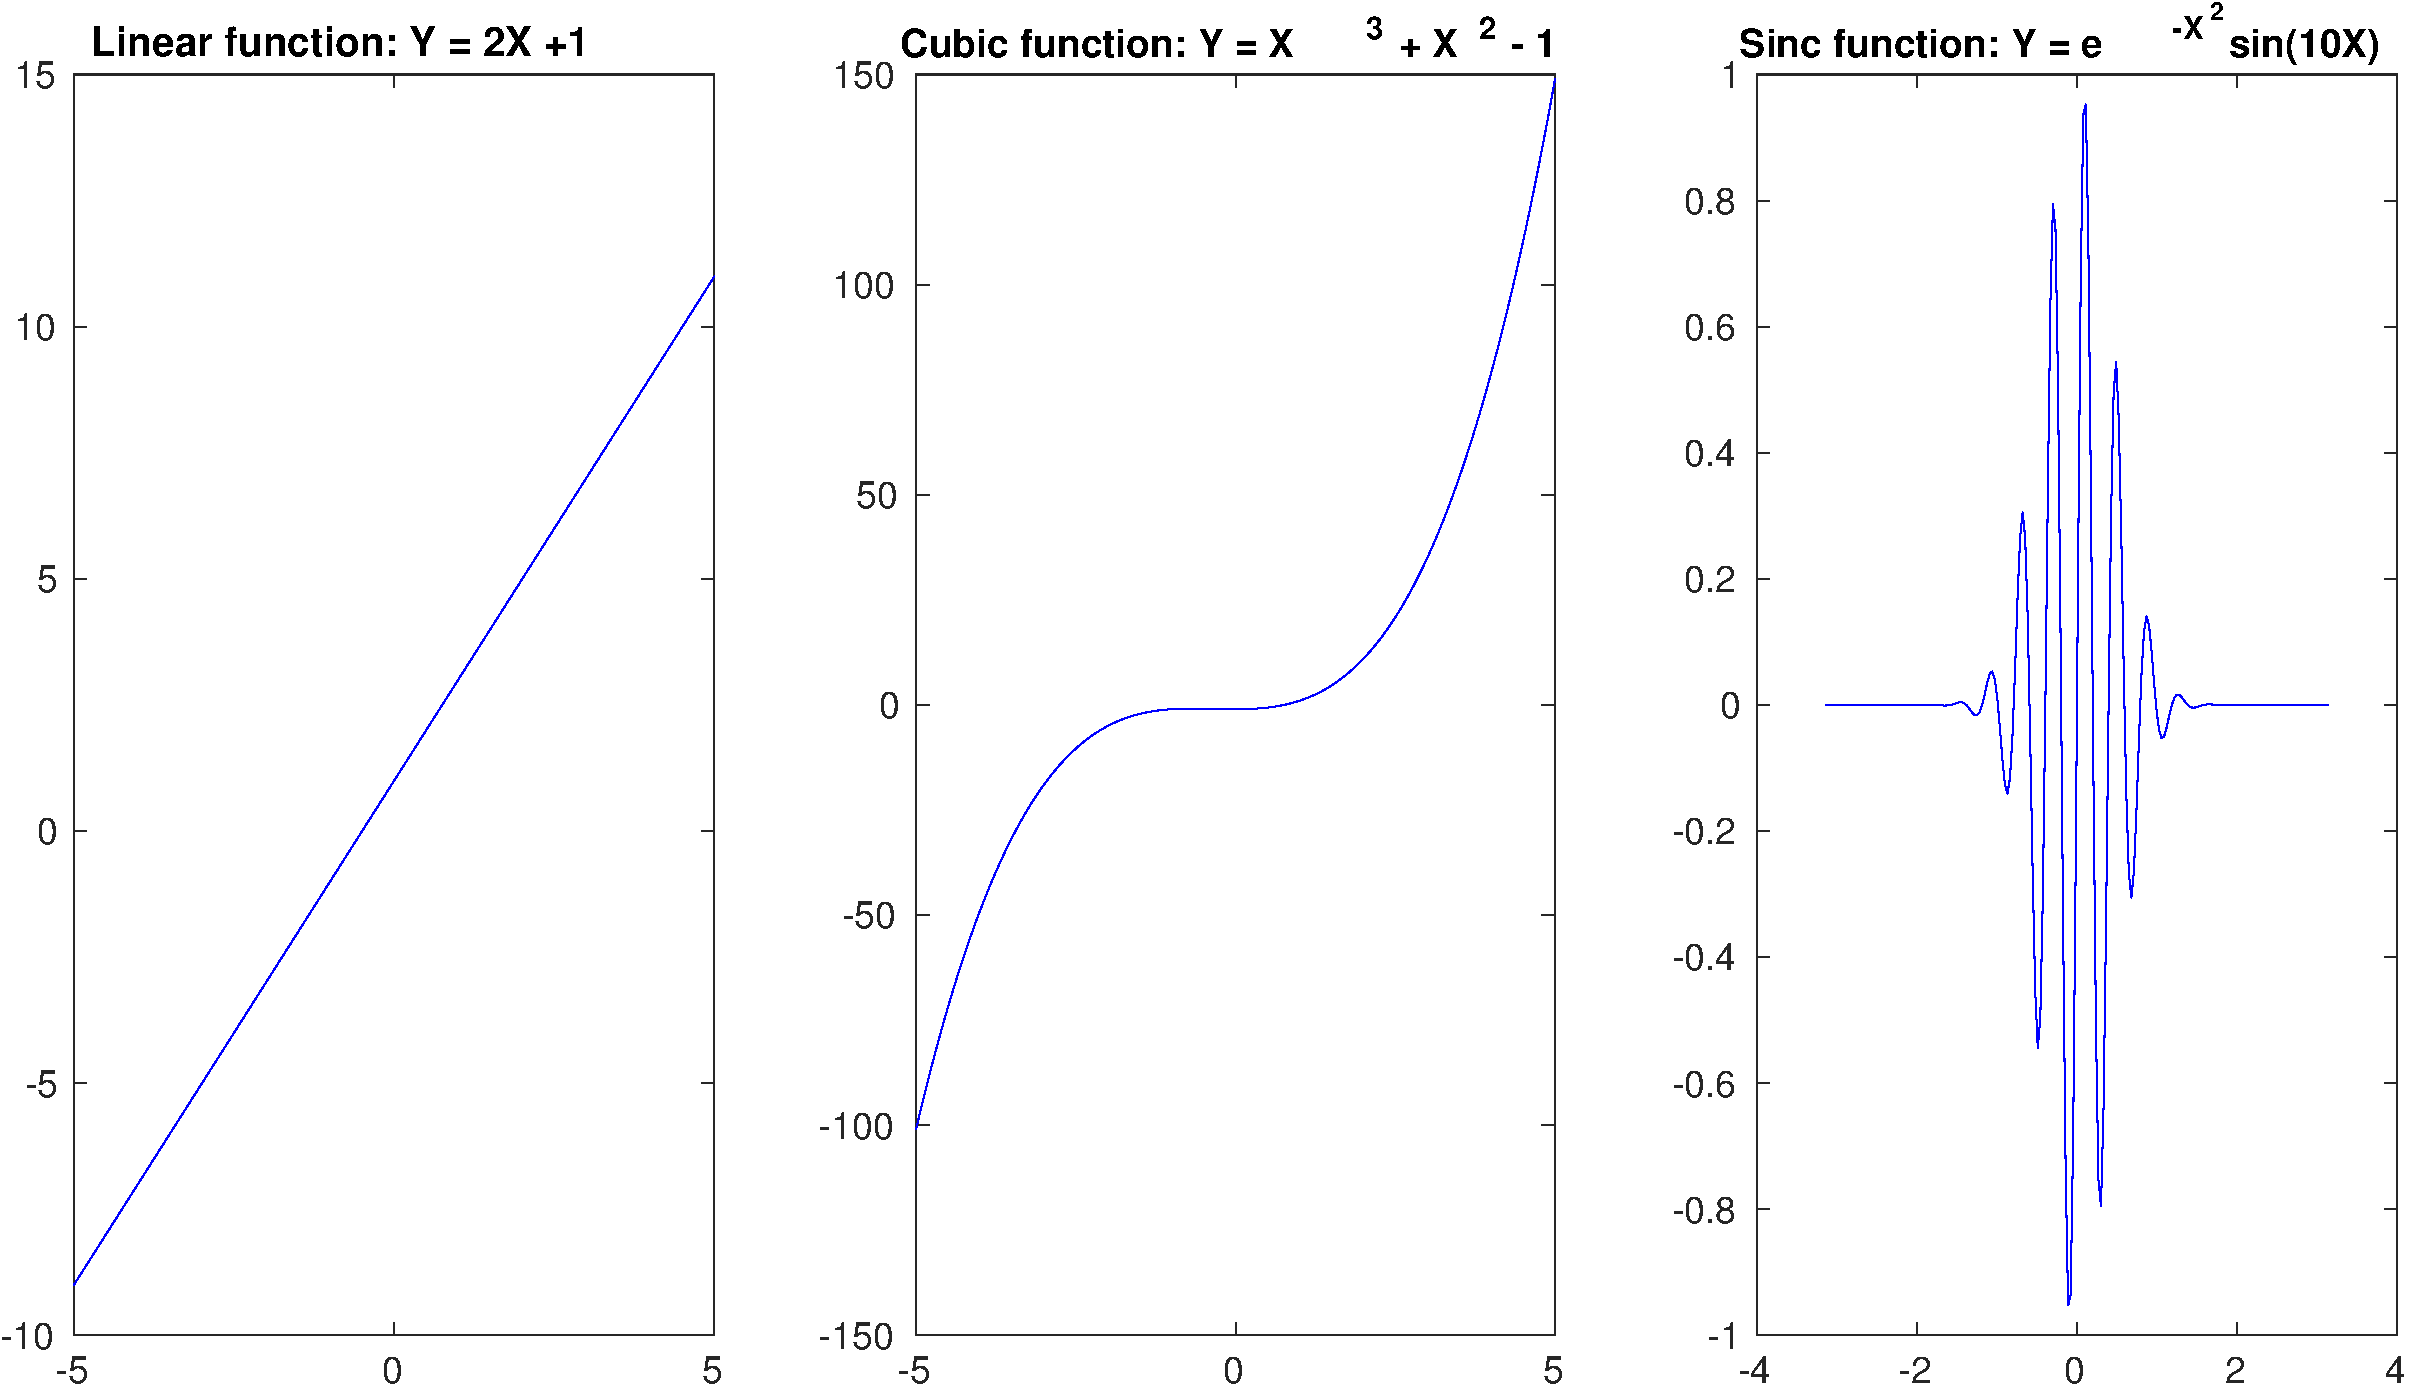
\includegraphics[scale=.40]{datasets.pdf}
    \caption{Functions to regress}
    \label{fig:regress_datasets}
\end{figure}

\subsection{Analysis}

For the linear and cubic functions, I got good results with polynomial
kernel of degree 1 and 3 respectively.

I did an extensive survey of the parameters for the first linear
model. On that particular model, the linear kernel seem to have
performed the best. Even for extremely low $\epsilon$ (eg
$\epsilon=0.005$), the number of support vectors needed to describe
the classifier is equal to two. Another obvious advantage of that
kernel was that no wiggle artefact appeared, in contrast with the
other more flexible kernels.

\begin{table}[H]
  \centering
  \begin{tabular}{l|r|r|r|r|r|r|r|r|r|r|}
\cline{2-11}
                                         & \multicolumn{5}{l|}{e value (Bound Inf)}                                                                                                 & \multicolumn{5}{l|}{Bound (e value 0.1)}                                                                                           \\ \cline{2-11} 
                                         & \multicolumn{1}{l|}{0.005} & \multicolumn{1}{l|}{0.01} & \multicolumn{1}{l|}{0.05} & \multicolumn{1}{l|}{0.1} & \multicolumn{1}{l|}{0.5} & \multicolumn{1}{l|}{0.01} & \multicolumn{1}{l|}{0.1} & \multicolumn{1}{l|}{1} & \multicolumn{1}{l|}{10} & \multicolumn{1}{l|}{100} \\ \hline
\multicolumn{1}{|l|}{Poly 1}             & 2                          & 2                         & 2                         & 2                        & 2                        & 20 **                     & 20 **                    & 13                     & 2                       & 100                      \\ \hline
\multicolumn{1}{|l|}{Poly 2}             & 3                          & 6                         & 6                         & 6                        & 3                        & 20 **                     & 20 **                    & 8                      & 3                       & 3                        \\ \hline
\multicolumn{1}{|l|}{Poly 3}             & 7                          & 7                         & 4                         & 4                        & 2 *                      & 20 **                     & 20 **                    & 15 *                   & 4 *                     & 4 *                      \\ \hline
\multicolumn{1}{|l|}{Poly 4}             & 5                          & 5                         & 5                         & 5                        & 4 *                      & 20 **                     & 20 **                    & 14 *                   & 5 *                     & 5 *                      \\ \hline
\multicolumn{1}{|l|}{RBF $\sigma^2=1$}   & 16                         & 7                         & 7                         & 4                        & 4 *                      & 20 **                     & 20 **                    & 20 **                  & 15 **                   & 4                        \\ \hline
\multicolumn{1}{|l|}{RBF $\sigma^2=0.5$} & 10                         & 9                         & 9                         & 7                        & 5 *                      & 20 **                     & 20 **                    & 20 **                  & 10 **                   & 7 *                      \\ \hline
  \end{tabular}
  \caption{Number of support vectors required for different kernels and parameters (*: wiggle artefact visible, **: function estimation completely off)}
  \label{table:dataset_lin}
\end{table}

% \begin{figure}[H]
%     \centering
%     \includegraphics[scale=.40]{two_gaussians.pdf}
%     %\caption{Two gaussians classification}
%     \label{fig:two_gaussians}
% \end{figure}

\section{Sum of Cosines}

\section{Hyper-parameter Tuning}


% \begin{figure}[H]
%     \centering
%     \begin{subfigure}{.5\textwidth}
%       \centering
%       \includegraphics[width=0.9\linewidth]{1-2-1-kernel7.png}
%       \caption{Support vectors reduce dataset}
%       \label{fig:ker7reduced}
%     \end{subfigure}%
%     \begin{subfigure}{.5\textwidth}
%       \centering
%       \includegraphics[width=0.9\linewidth]{1-2-1-kernel7spiral.png}
%       \caption{No compression}
%       \label{fig:ker7spiral}
%     \end{subfigure}
%     \caption{Support vectors}
%     \label{fig:ker7}
% \end{figure}

\section{Application of the Bayesian framework}

\section{Robust regression}

\section{Applications}

\bibliographystyle{ieeetr} \bibliography{bib-db}
\end{document}
